\documentclass[a4paper,11pt]{article}
\usepackage{graphicx}
\pagestyle{empty}
\title{TestSort vs 1.0}
\author{Saswat Raj}
\begin{document}
\maketitle
\newpage
\section{User Manual}
\subsection{Overview} TestSort is a command line utility that compares the sorting time taken by the various sort procedures (currently heapsort,mergesort,bubblesort and quicksort) according to the user input of range and other details and plots them onto a graph using the gnuplot utility for linux.
\subsection{Dependencies}
\begin{itemize}
\item Linux 
\item gcc compiler 
\item bash shell
\item gnuplot utility
\end{itemize}
\subsection{System Specifications} The user should add the path of the testsort.sh file to the path variable to access the command from anywhere in the command line. It is necessary that the file has the permissions to read and write data to the system.The \emph{src} folder should be the child of the directory containing the testsort file.The testsort.sh should be executable and so should the files be in the src directory.If the files are not executable use the \emph{chmod} command to make them executable.
\subsection{User Command} To use the testsort function use the command line in linux environment.If the directory of testsort is already in your path then you can directly provide your specifications by using the command :\begin{verbatim}
./testsort -i init -r res -f final -a avg -o outputfile 
           -s [heap,merge,quick,bubble]
\end{verbatim}
where:\begin{itemize}
\item init :initial value to start testing from
\item res :increment per step of the calculation
\item final :the final value of the calculation
\item avg :the numeber for tavg calculation
\item -s\ldots :the sorts to be tested
\end{itemize}
\textbf{Note :}\emph{The -s option should be mentioned in at the last of the input specifications}
\newpage
\paragraph{The Calculation Of Data:}The program iterates over from \emph{init} to \emph{final} incremented by \emph{res} and the total time is calculated for \emph{avg} number of such calculations for given number of fixed data.The data is then sent to  \emph{gnuplot} for the corresponding output graph.The output file is stored in \emph{src} folder in the project directory.
\section{Developer Manual:}
\subsection{Structure of Files and their Uses:}
\begin{itemize}
\item testsort
\item src
\begin{itemize}
\item mergesort.c
\item heapsort.c
\item bubblesort.c
\item quicksort.c
\item merge.sh
\item bubble.sh
\item quick.sh
\item heap.sh
\item plot.sh
\item generate.c
\end{itemize}
\end{itemize}
\textbf{\emph{mergesort.c}}:Implements the mergesort algorithm.This generates merge executable during runtime that takes an argument the number of elements in array to sort.\\
\textbf{\emph{heapsort.c}}:Implements the heapsort algorithm.This generates heap executable during runtime that takes an argument the number of elements in array to sort.\\
\textbf{\emph{bubblesort.c}}:Implements the bubblesort algorithm.This generates bubble executable during runtime that takes an argument the number of elements in array to sort.\\
\textbf{\emph{quicksort.c}}:Implements the quicksort algorithm.This generates quick executable during runtime that takes an argument the number of elements in array to sort.\\
\textbf{\emph{merge.sh}}:Returns the average time taken by the merge procedure over the generated number of elements. It takes as arguments the average number of times and the number of values in the array.\\
\textbf{\emph{heap.sh}}:Returns the average time taken by the heap procedure over the generated number of elements. It takes as arguments the average number of times and the number of values in the array.\\
\textbf{\emph{bubble.sh}}:Returns the average time taken by the bubble procedure over the generated number of elements. It takes as arguments the average number of times and the number of values in the array.\\
\textbf{\emph{quick.sh}}:Returns the average time taken by the quick procedure over the generated number of elements. It takes as arguments the average number of times and the number of values in the array.\\
\textbf{\emph{plot.sh}}:Uses the gnuplot to plot the data from output file to gnuplot and displays it on the screen.\\
\textbf{\emph{generate.c}}:Generates the executable gen which takes as arguments the required random numbers to generate and places them in an output file \emph{tempfile.txt}.\\
\subsection{Files Generated during runtime :}
\begin{itemize}
\item src:merge
\item src:heap
\item src:quick
\item src:bubble
\item src:gen (generates random numbers)
\item src:\emph{output file}
\end{itemize}
\subsection{Testsort:}Testsort uses getopt to parse arguments and the -s argument is processed last by shifting the argument index to the very end.It replaces the default values by the values mentioned in the initial arguments after checking for the validity of the arguments.It then generates the C executables if they are not present and runs according to the instructions specified and generates the output file and the gnuplot
\newpage
\section{Sample Working:}
\begin{figure}[ht!]
\centering
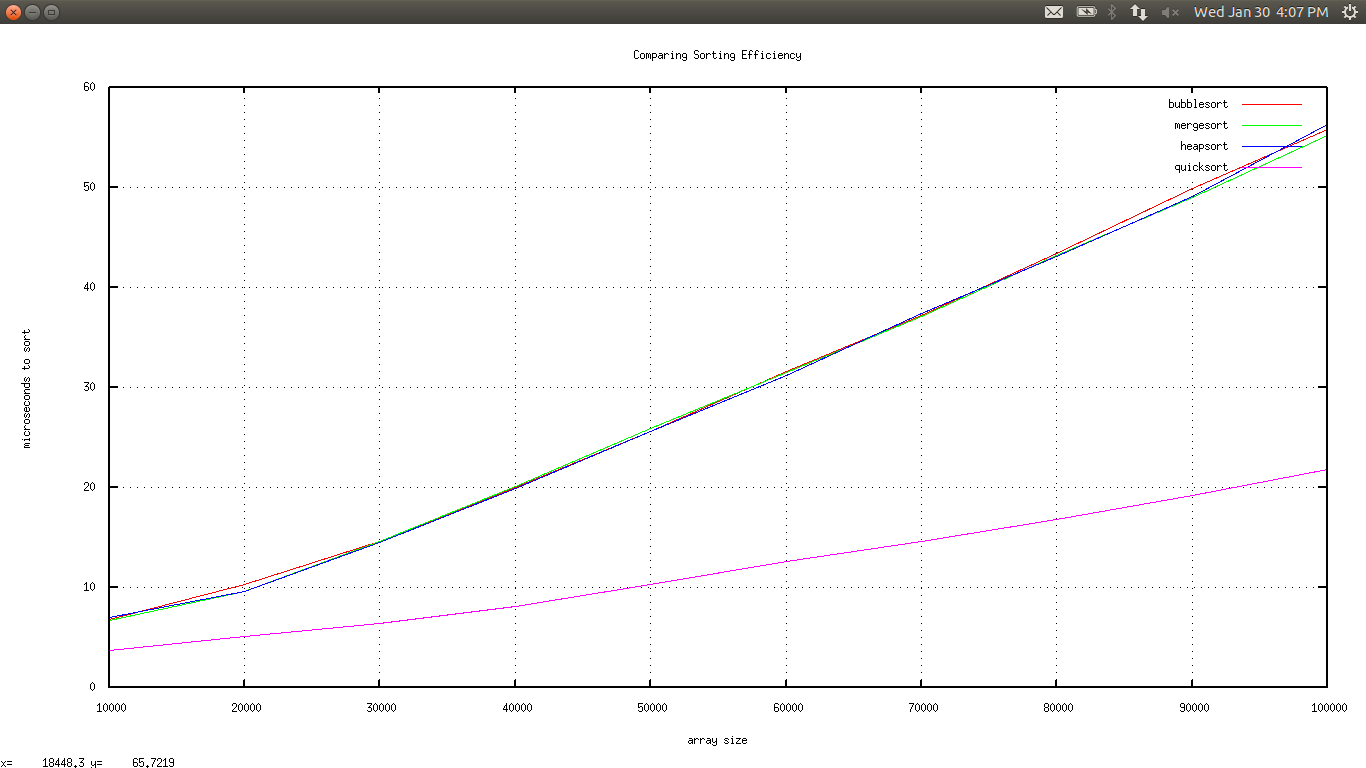
\includegraphics[width=120mm]{output.png}
\caption{The Graph for larger values when plotted in seconds}
\label{output1}
\end{figure}
\begin{figure}[ht!]
\centering
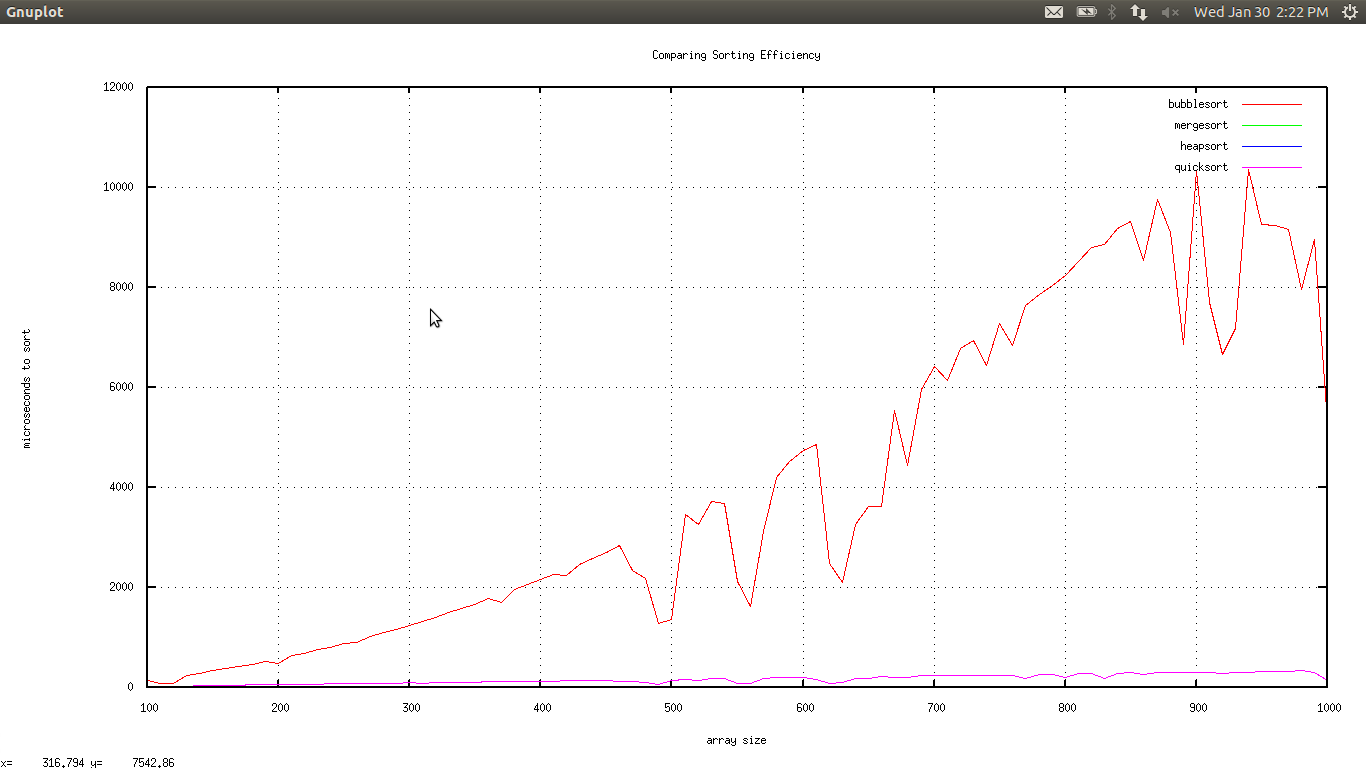
\includegraphics[width=120mm]{output1.png}
\caption{The Graph for smaller values when plotted in microseconds}
\label{output}
\end{figure}
\begin{figure}[ht!]
\centering
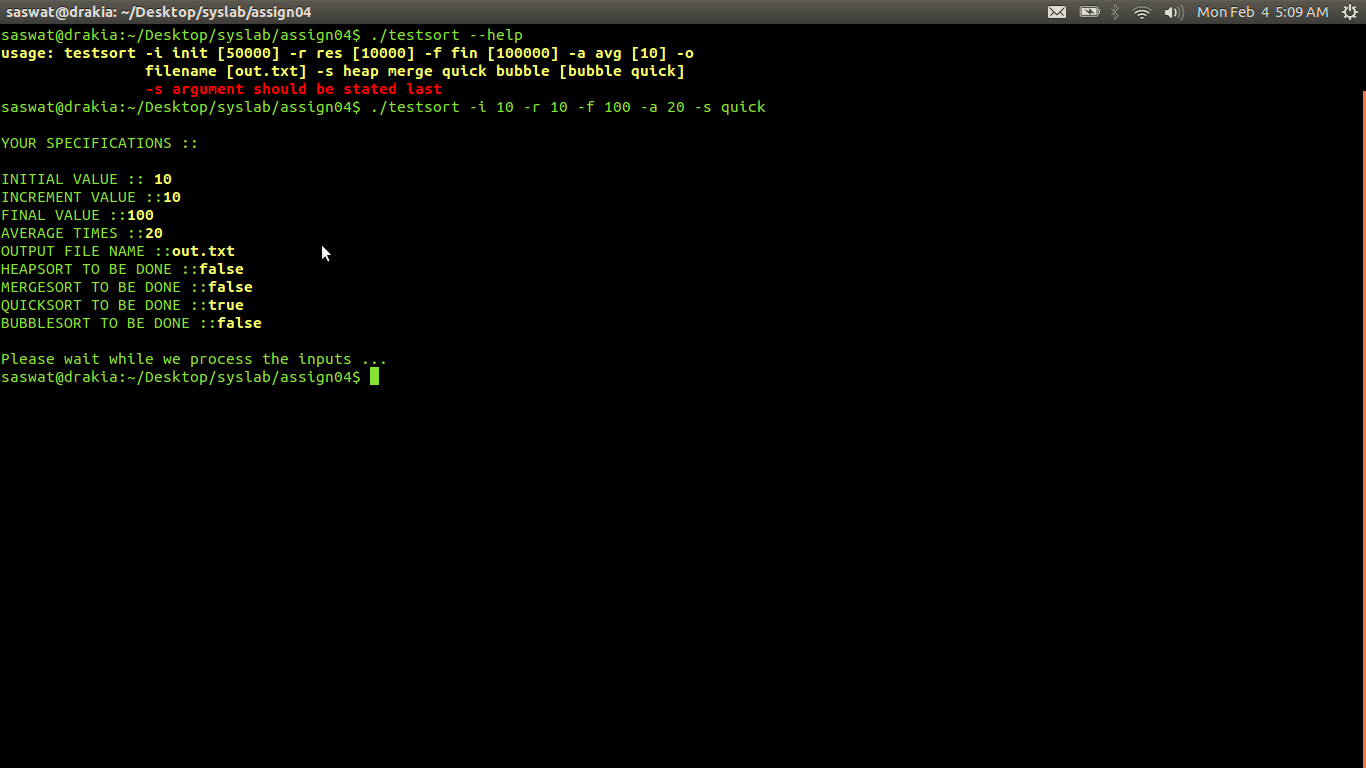
\includegraphics[width=120mm]{output3.png}
\caption{Using command in command line}
\label{output3}
\end{figure}
\end{document}
